\documentclass[11pt]{article}

% Change "review" to "final" to generate the final (sometimes called camera-ready) version.
% Change to "preprint" to generate a non-anonymous version with page numbers.
\usepackage[review]{acl}

% Standard package includes
\usepackage{times}
\usepackage{latexsym}

% For proper rendering and hyphenation of words containing Latin characters (including in bib files)
\usepackage[T1]{fontenc}
% For Vietnamese characters
% \usepackage[T5]{fontenc}
% See https://www.latex-project.org/help/documentation/encguide.pdf for other character sets

% This assumes your files are encoded as UTF8
\usepackage[utf8]{inputenc}

% This is not strictly necessary, and may be commented out,
% but it will improve the layout of the manuscript,
% and will typically save some space.
\usepackage{microtype}

% This is also not strictly necessary, and may be commented out.
% However, it will improve the aesthetics of text in
% the typewriter font.
\usepackage{inconsolata}

%Including images in your LaTeX document requires adding
%additional package(s)
\usepackage{graphicx}
\usepackage{booktabs}

% If the title and author information does not fit in the area allocated, uncomment the following
%
%\setlength\titlebox{<dim>}
%
% and set <dim> to something 5cm or larger.

\title{A Bounded Coordination-Support Capability for Multi-Party Settings: Task-State Monitoring in Firefighter Incident Command}

% Author information
\author{David Grünert \and Barbara Morgenstern \and Florian Peczinka \\
\textbf{\and Dario Holenstein \and Roland Brunner \and Alexandre de Spindler} \\
Zurich University of Applied Sciences, Winterthur, Switzerland \\
\texttt{\{grud,morgebar,pecziflo,holendar,desa\}@zhaw.ch} \\
Freiwillige Feuerwehr Stadt Zug, Zug, Switzerland \\
\texttt{roland.brunner@stadtzug.ch}}


\begin{document}
\maketitle
\begin{abstract}
  Many coordination settings require digital support systems for several humans who coordinate through shared state and ongoing communication. We study one such application in firefighter incident command: a dashboard that monitors the state of predefined operational tasks from radio transcripts.
  Building such a dashboard raises a practical design question: how much transcript structure is actually needed for LLM-based task-state monitoring? Rich transcript structure may require speaker diarization, speaker-change detection, or semantically refined utterance segmentation, all of which are difficult to obtain reliably from radio communication and can add complexity and latency.
  We evaluate this question on source-grounded synthetic firefighter scenarios under transcript conditions that vary speaker identity and utterance boundaries, with incremental inference as the deployment-facing condition and full-transcript inference as an offline reference.
  Across repeated runs, incremental monitoring remains strong across all transcript conditions. Differences between transcript structures are small, continuous transcripts remain competitive, and the main weaknesses are identifying the responsible unit and capturing the completion result, which remain broadly similar across conditions.
  These results suggest that for this bounded dashboard-support capability, neither speaker identities nor semantically precise utterance boundaries are a primary requirement in the controlled setting studied here.
\end{abstract}

\section{Introduction}
\label{sec:introduction}

Large language models are now widely used in bilateral settings such as chat assistants and individual copilots \citep{Maedche2019,Nah2023}. Yet many real work settings require digital support for several humans who coordinate through ongoing communication and maintain a shared operational picture rather than seek isolated answers. Recent work on human-AI collaboration therefore argues for moving beyond assistant-centric interaction toward AI systems that support team processes and shared coordination \citep{Seeber2020,Anthony2023,Bankins2024}. In mission-critical domains, one concrete support need is to maintain an explicit view of what has been assigned, what remains pending, and what has been completed.

Firefighter incident command provides a concrete instance of this broader problem. Commanders coordinate multiple units through short, interleaved radio transmissions while tracking operational tasks. We study this setting through a command-support dashboard whose task list is already derived from procedures and incident context. The model does not discover new tasks or make operational decisions. Instead, it proposes conservative state updates for predefined tasks under human oversight.

Once such a dashboard is the target system, a more specific technical question becomes central: how much transcript structure is actually needed for LLM-based task monitoring from multi-party radio traffic? Rich transcript structure may be costly or brittle to obtain in this setting. Speaker identity may require diarization or prior speaker models, both of which remain difficult under noisy multi-speaker conditions and heterogeneous channels \citep{Mehrish2023A}. Utterance boundaries may be supplied by voice activity detection, but pause-based segmentation can split incomplete thoughts, while more refined speaker-change or semantic segmentation adds models, engineering effort, and delay \citep{Mehrish2023A}. For a command-support system, these are not cosmetic transcript properties but potential deployment bottlenecks because real-time speech systems must trade off model complexity against latency and computational load \citep{Michelsanti2020An}.

This motivates the central research question of the paper: \emph{how much transcript structure is actually needed to track predefined task state reliably from ongoing multi-party communication in this operational setting?} More concretely, we ask whether task-state monitoring depends on speaker identities and explicit utterance boundaries, or whether a simpler transcript representation suffices for this monitoring task.

We address this question through a controlled evaluation of closed-world task-state monitoring across transcript conditions that vary speaker identity and utterance boundaries while keeping the underlying scenario content fixed. The paper contributes in three ways. First, we formulate a bounded coordination-support problem centered on monitoring the state of known operational tasks in firefighter incident command. Second, we introduce a source-grounded synthetic dataset construction and validation pipeline that enables controlled comparison of transcript-structure effects while holding operational content constant. Third, we report results for incremental monitoring and a secondary offline full-transcript reference in a reproducible evaluation pipeline with auditable artifacts and deterministic tests\footnote{GitHub repository with complete data, code and results not revealed due to anonymisation}.

% Update footnote to: https://github.com/zhaw-iwi/swisstext26_pub

The remainder of the paper is structured as follows. Section~\ref{sec:background} situates the work in the literature on multi-human AI support and facilitation. Sects.~\ref{sec:application}--\ref{sec:experimental-setup} then cover the application framing, dataset, and experimental design, before Sect.~\ref{sec:evaluation} reports the results and Sect.~\ref{sec:conclusion} concludes.

\section{Background}
\label{sec:background}

This section situates the paper at the intersection of multi-human AI support and team information-processing support. It motivates why a dashboard-centered command-support system can be understood as one instance of a broader class of digital support systems for shared coordination, and why task-state monitoring is a meaningful bounded capability within that class.

A large share of current generative AI applications remains focused on the individual user: question answering, drafting, summarisation, or recommendation for a single human operator \citep{Maedche2019,Nah2023}. By contrast, many work settings require models to interpret contributions distributed across several people, maintain state over time, and support shared rather than individual understanding. Reviews of human-AI teaming show that much of the literature still focuses on bilateral assistants, dyads, or otherwise narrowly scoped team configurations \citep{Lyons2021,ONeill2022,Anthony2023,Bankins2024}. This leaves open how AI systems should support shared state and coordination across ongoing multi-party interaction through a shared artefact such as a dashboard.

Research on Group Support Systems has long shown that collaboration quality depends not only on who contributes, but also on how information is processed and coordinated within the group \citep{Nunamaker1991,DennisValacich1993,DennisWixomVandenberg2001,Briggs2003}. Facilitation has been central in this tradition because groups systematically suffer from process losses such as production blocking, dominance effects, incomplete information pooling, and premature convergence \citep{StasserTitus1985,DennisValacich1993,Briggs2003}. Recent work on AI in teams suggests that digital artefacts may take over selected support capabilities, especially those involving consistency, timing, monitoring, or large-scale information processing, while humans retain judgement, legitimacy, and contextual authority \citep{Dellermann2019HI,Seeber2020,DennisLakhiwalSachdeva2023}.

Our paper focuses on one such capability: maintaining an explicit representation of task state from ongoing multi-party communication. In facilitation terms, this is primarily an information-processing support function. The command-support system does not replace operational decision making. Rather, it externalises on the dashboard what the team has already established: which tasks have been handed out, which unit appears responsible, which tasks have been completed, and what completion result has been reported.

Technically, this formulation is related to dialogue state tracking and information extraction. Dialogue state tracking maintains structured state representations from dialogue history in task-oriented systems \citep{Balaraman2021DSTSurvey}. Information and event extraction similarly recover structured records, events, or arguments from text, often against predefined schemas \citep{ChambersJurafsky2011,XiangWang2019EventSurvey}. Our setting differs in that the state variables are predefined SOP- and procedure-related operational tasks, the evidence is distributed across multi-party radio communication, and the output is used for incremental dashboard support rather than autonomous dialogue management or open-ended event discovery.

We study this capability in a deliberately bounded operational setting rather than in the most open-ended form of multi-human coordination. If a digital support system cannot reliably maintain assignment and completion state for predefined tasks, then more advanced functions such as summarisation, blind-spot detection, or process coaching are unlikely to be trustworthy. Conversely, if task-state monitoring proves robust under reduced transcript structure, this suggests that at least some multi-human information-processing functions may not require expensive preprocessing pipelines.

Taken together, these strands motivate AI support for shared coordination, but they do not yet answer the more specific deployment question studied in this paper: how much transcript structure is required for closed-world task-state monitoring from ongoing multi-party communication? Firefighter incident command is a useful case because the dashboard-centered support function is operationally meaningful, the communication is genuinely multi-party, and transcript enrichment can be costly. For a bounded function such as digital task-state tracking, richer transcript preprocessing may help, but it is not obvious that speaker labels and clean utterance boundaries are necessary.

\section{Application Context and Requirements}
\label{sec:application}

Firefighter incident command provides a concrete example of the broader class of multi-human digital support settings outlined in the previous section. In this setting, the command-support system is not meant to converse with a single user in isolation. Instead, it supports shared coordination by helping incident command maintain an explicit, inspectable view of operational task state as evidence arrives through multi-party radio traffic. We use this case not as the whole claim of the paper, but as a demanding setting from which to derive requirements for one bounded coordination-support capability.

\subsection{Application Setting}

The user-facing surface is a dashboard that presents the task list together with current task status and recent communication context, as illustrated in Figure~\ref{fig:dashboard}. Its role is to reduce memory burden and preserve an explicit overview of open and completed tasks. The dashboard thus serves as the interface of a bounded information-processing support system for the command team. It helps keep tasks from getting lost in noisy, interleaved, time-critical radio communication.

\begin{figure*}[t]
  \centering
  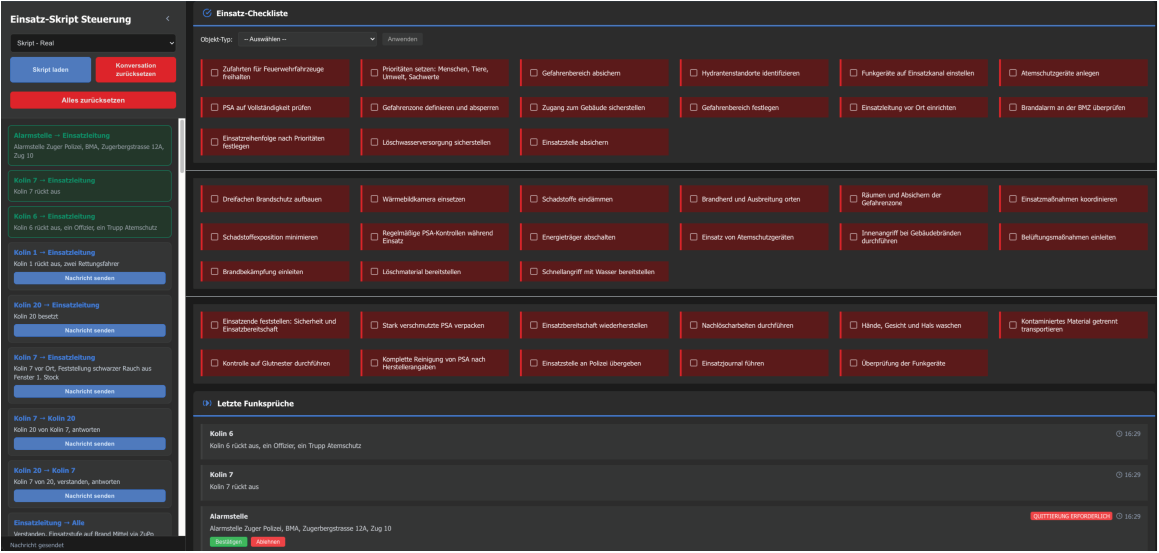
\includegraphics[width=\textwidth]{figures/figure_dashboard.png}
  \caption{Dashboard interface of our command-support system.}
  \label{fig:dashboard}
\end{figure*}

Figure~\ref{fig:workflow} situates this dashboard within our implemented command-support system. In the operational setting, predefined tasks originate from procedures and incident context, for example from baseline checklists associated with the incident type, from object-specific information, and from a building register. This information is available and selected at dispatch time. Radio communication then provides the dynamic evidence for whether those tasks have been assigned to firefighter units, acknowledged, and completed. The present paper therefore treats task-state monitoring as a closed-world problem: the task set is supplied in advance, and transcript evidence is used to update task state.

This application framing is also consistent with lightweight qualitative feedback from a prototype demonstration of our command-support system with active firefighters. Beyond transcript capture itself, they emphasized the value of temporal tracking features, such as seeing how long a task has remained open or how long a crew has been silent. We treat this feedback as informal practitioner grounding rather than as a formal user-study result.

\begin{figure*}[t]
  \centering
  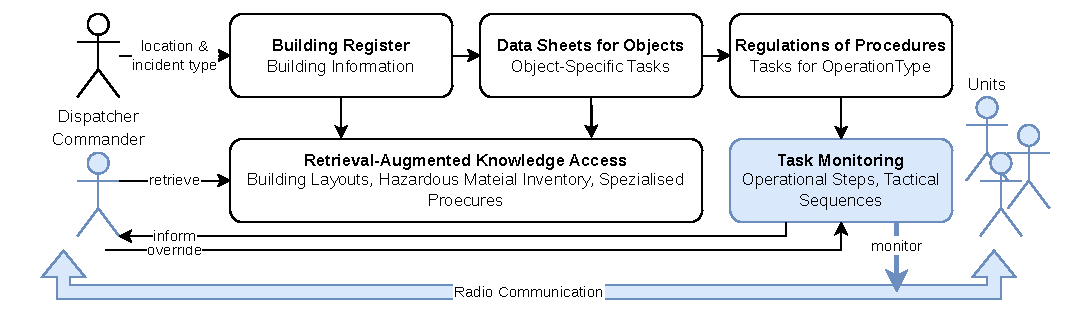
\includegraphics[width=0.92\textwidth]{figures/figure_workflow.pdf}
  \caption{Operational flow of our command-support system, with dashboard components shown in blue.}
  \label{fig:workflow}
\end{figure*}

\subsection{Monitoring Problem}

Emergency radio communication differs substantially from the dialogue structure often assumed in conversational NLP. Messages are short, domain-specific, and often elliptical. Operational meaning is distributed across acknowledgements, updates, and follow-up reports rather than contained in a single self-sufficient utterance. For the command-support system, useful support therefore depends on reconstructing task state from distributed conversational evidence rather than isolated turns.

This creates the concrete design pressure behind our research question. If the dashboard requires speaker identities, the implementation may depend on diarization or prior speaker models despite radio-channel noise and changing crews \citep{Mehrish2023A}. If it requires semantically well-formed utterance boundaries, pause-based segmentation may be insufficient and additional speaker-change or semantic segmentation steps may be needed before task monitoring can run \citep{Mehrish2023A}. These components increase engineering effort and add latency, which is a relevant concern in real-time speech systems that must trade off model complexity against computational load \citep{Michelsanti2020An}. In our setting, such components may fail precisely in the noisy conditions where operational support is most valuable. We therefore investigate how much structure the transcript representation actually needs for this monitoring task. More broadly, the firefighter case can thus be understood as one example of a digital support system that performs a bounded, process-relevant information-processing function inside a human team.

\subsection{System Requirements}

The command-support system must monitor the state of predefined operational tasks supplied from procedures and incident context. The scope is therefore closed-world monitoring of known tasks rather than open-ended task discovery.

The command-support system must operate under explicit human oversight. Proposed task-state updates must remain transparent to the command team and be subject to human confirmation or override.

The command-support system must support near-real-time dashboard updates during ongoing incidents. Task-state information must be revised as new communication evidence becomes available so that the dashboard remains a current operational overview.

\subsection{Task Formulation}

These application requirements lead to a closed-world task formulation. For each predefined task $\tau$ and each discrete prefix index $k$, the model outputs a structured task-state prediction
\[
y(\tau, k) = (a, u, c, o).
\]
Here, $k$ denotes the current transcript prefix, that is, the communication evidence available up to that point. The tuple components correspond to \texttt{assigned}, \texttt{assigned\_unit}, \texttt{completed}, and \texttt{completion\_outcome}, respectively. \texttt{assigned} (boolean) indicates whether the transcript provides evidence that responsibility for the task has been assigned to a unit and acknowledged. \texttt{assigned\_unit} (nullable string) indicates which unit is identified as responsible for the task. \texttt{completed} (boolean) indicates whether the transcript provides evidence that the task has been completed. \texttt{completion\_outcome} (nullable string) captures the reported completion result or completion evidence in short textual form.

\section{Dataset}
\label{sec:dataset}

We evaluate the monitoring formulation on a controlled synthetic dataset. The synthetic design is deliberate: the research question requires the same underlying operational scenario to be rendered under different transcript-structure conditions while keeping task content fixed. A source-grounded synthetic dataset makes this possible, allowing differences between transcript conditions to be attributed to representation rather than scenario content.

\subsection{Source-Grounded Construction}

The dataset was constructed with a prompt-based generation and validation pipeline grounded in three source types: Swiss radio-procedure material\footnote{Bundesamt für Bevölkerungsschutz, Funkmaterial Sprechregeln, February 2004}, a real firefighter communication transcript used for surface realism, and canonical procedural regulations\footnote{Feuerwehr Koordination Schweiz FKS, Reglement Einsatzführung, November 2022}. These materials were distilled into source notes used for both scenario generation and validation.

Each scenario was generated as a fixed-schema JSON object containing an ordered message sequence, a closed-world list of predefined tasks, and gold task states. In addition to the final task state, each gold entry stores the message id at which assignment first becomes valid and, when applicable, the message id at which completion first becomes valid. Task-command linkage is annotation-grounded rather than based on lexical overlap between task labels and command wording. This enables deterministic derivation of gold states for every incremental transcript prefix.

Validation was performed in two independent rubric-guided passes: a structural pass for radio style and protocol coherence, and a content pass for operational plausibility, role-task alignment, task sequencing, and traceability of gold states to explicit message evidence. We implemented both dataset generation and validation with \texttt{gpt-5.4} as a bounded LLM judgment process under source-grounded constraints \citep{Zheng2023,Rotteger2024SafetyPrompts}. This source-grounded generation-and-judge setup was used to make the synthetic data more representative of the intended application setting while preserving control over transcript-structure variation. The generation--validation--revision loop ran for 12 rounds until the dataset passed both validation streams.

As an additional plausibility check, the extracted structure and resulting scenarios were reviewed within the team. They were judged to align with observed communication structures and contents from the intended application setting. While informal and not a formal annotation study, this review provides additional support for the dataset's plausibility as a set of realistic scenarios.

\subsection{Dataset Contents}

The final dataset contains five German-language firefighter scenarios with 102 ordered radio messages and 15 predefined tasks in total. Every scenario contains exactly three monitored tasks, yielding 15 task-state traces overall. All 15 tasks are explicitly assigned in the transcript evidence, 12 are completed within the scenario, and 3 remain assigned but incomplete at scenario end.

The five scenarios cover a kitchen fire in an apartment building, an underground-garage fire, a school basement fire, a workshop fire involving gas cylinders, and an attic fire in a row house. Across these scenarios, the monitored task families include water supply, search, ventilation, suppression, access control, gas-cylinder cooling, CO measurement, and final control. The assigned units include command-relevant firefighter roles such as \texttt{Angriffstrupp}, \texttt{Wassertrupp}, \texttt{Messgruppe}, \texttt{Kontrolltrupp}, and \texttt{Verkehrstrupp}.

\subsection{Representation and Limitations}

Each scenario stores ordered messages, predefined tasks, and one final gold state per task, using the same output fields as the monitoring model: assignment status, assigned unit, completion status, and optional completion outcome. For incremental evaluation, per-prefix gold states are derived deterministically from the stored assignment and completion transition ids.

These gold task states serve as the reference labels for evaluation, and the stored transition ids define the gold assignment and completion points used in incremental detection metrics.
For evaluation, these fields also induce the three-way task state \texttt{NOT\_ASSIGNED}/\texttt{ASSIGNED}/\texttt{COMPLETED}.

Before evaluation, all scenario files pass deterministic local validation checks for schema conformance, sequential message ids, exact alignment between predefined tasks and gold task states, and consistency constraints on assignment/completion labels.

The limitations of the study follow directly from this dataset design and should be read upfront. The dataset is synthetic, small, and intentionally controlled. The scenarios are cleaner and more linear than real firefighter radio traffic, with limited protocol noise, dispatch and handover tails, and some bundled tasks that compress multi-step work into a single monitored item. The evaluation also begins from text transcripts rather than raw audio, so it does not include upstream speech-recognition or radio-channel degradation effects. Finally, the task formulation is deliberately narrow: it tests closed-world monitoring of predefined tasks, not open-ended task discovery or broad operational performance. We therefore use the dataset as controlled evidence for transcript-structure sensitivity in dashboard-oriented task monitoring, not as a realism corpus or a direct deployment claim.

\section{Experimental Setup}
\label{sec:experimental-setup}

We evaluate the dataset under a $3 \times 2$ design that varies transcript structure and processing mode while keeping the underlying scenario content fixed.

\subsection{Conditions}

We compare three transcript structures: \textbf{structured\_dialogue}, which includes speaker identities and utterance boundaries, \textbf{no\_speaker}, which retains utterance boundaries but omits speakers, and \textbf{continuous\_transcript}, which contains neither speakers nor boundaries. This last condition approximates the minimum structure available when speakers cannot be identified and reliable utterance segmentation is not available.

We evaluate two processing modes: \textbf{incremental}, which predicts on each growing message prefix from the first message to the full transcript, and \textbf{full\_transcript}, which predicts once on the complete transcript.

Incremental processing is the primary application condition. The \texttt{full\_transcript} condition serves as a secondary offline reference once all evidence is available. For incremental \texttt{continuous\_transcript} mode, each prefix is rendered as one continuous text string without speaker labels or message boundaries.

\subsection{Execution and Reproducibility}

All reported values are batch-level means across 12 repeated runs. The notebook runs the evaluation in live mode with \texttt{gpt-5.2} at temperature 0.0. Repeated runs are reported because live API inference can still show small residual variation despite deterministic settings. The evaluation prompt instructed the model to behave conservatively: when the transcript did not provide sufficient evidence for assignment or completion, the corresponding fields were to remain \texttt{false}/\texttt{null}. This reflects the operational preference to avoid overstating task progress under incomplete evidence. The evaluation pipeline persists each request and response artifact using deterministic identifiers over run, scenario, structure condition, processing mode, and prefix index, supporting resume-safe execution and auditability. The repository contains the dataset-generation prompts, validation prompts, source notes, evaluation prompt payloads, and persisted request/response artifacts. The tables report 95\% confidence intervals from the batch summaries exported by the notebook and evaluation code.

\subsection{Metrics}

We report four state-monitoring metrics in both processing modes. In the incremental setting, each metric is computed at every evaluated prefix and then averaged over prefixes. In the \texttt{full\_transcript} setting, the same metric is computed once on the final scenario transcript.

\textbf{Assignment accuracy.} This metric measures, for each predefined task, whether the predicted \texttt{assigned} value matches gold.

\textbf{Unit assignment accuracy.} This metric measures whether the predicted \texttt{assigned\_unit} matches gold. It is evaluated on tasks for which either gold or prediction marks the task as assigned, so that unit assignment is scored only where a responsible unit is relevant. In the incremental setting, scores are first computed per prefix and then averaged. Prefixes without any unit-assignment support contribute 0.0 by construction.

\textbf{Completion accuracy.} This metric measures, for each predefined task, whether the predicted \texttt{completed} value matches gold.

\textbf{State accuracy.} This metric collapses each task state to one of \texttt{NOT\_ASSIGNED}, \texttt{ASSIGNED}, or \texttt{COMPLETED}, and then measures whether the predicted three-way state matches gold.

For incremental evaluation, we additionally report assignment and completion detection latency together with assignment and completion miss rate. The gold transition points come from explicit scenario annotations for first assignment and, when applicable, first completion evidence. Assignment is anchored to the first operative command that hands responsibility for the predefined task to the assigned unit. Later refinements to the same unit do not reset the assignment point.

\textbf{Assignment detection latency.} This metric measures the number of prefix steps between the gold assignment point and the first prefix at which the model predicts the task as assigned with the correct unit. It is reported only for successfully detected assignment events.

\textbf{Completion detection latency.} This metric measures the number of prefix steps between the gold completion point and the first prefix at which the model predicts the task as completed while preserving assigned state and the correct unit. It is reported only for successfully detected completion events.

\textbf{Assignment detection miss rate.} This metric is the proportion of gold assignment events that are never correctly detected before the scenario ends.

\textbf{Completion detection miss rate.} This metric is the proportion of gold completion events that are never correctly detected before the scenario ends.

\textbf{Terminal gaps.} As a reference comparison, we report terminal assignment, unit-assignment, completion, and state gaps. These are the absolute differences between the last incremental-prefix metrics and the corresponding \texttt{full\_transcript} metrics for the same run, scenario, and transcript structure.

\textbf{Completion outcome.} For \texttt{completion\_outcome}, exact match proved too strict because the model often paraphrases the completion evidence rather than reproducing the gold message string verbatim. We therefore report a retrospective similarity-based reanalysis on gold-completed tasks using ROUGE-L F1 as a secondary reference metric.

\section{Results}
\label{sec:evaluation}

The main empirical result is straightforward: in this controlled setup, simplifying transcript structure has little effect on aggregate task-state monitoring performance. Across all conditions, assignment, completion, and current-state accuracy remain high. The lowest aggregate metric is unit assignment, but this should be interpreted as a stricter prefix-level score rather than as frequent confusion between responsible units.

\subsection{Incremental Accuracy}

Incremental inference is the more deployment-relevant setting because the command-support system must update task state while communication unfolds. Table~\ref{tab:incremental-results} shows that performance remains strong and tightly clustered across transcript structures. The unit-assignment column is consistently lower than the other state-tracking metrics, but inspection of the persisted artifacts suggests that this does not primarily reflect wrong responsible-unit names. Most unit mismatches arise when an incremental prediction has not yet marked a gold-assigned task as assigned, especially for conditional or preparatory tasking, with a smaller number of premature assignments. Thus, the harder part is aligning assignment timing and unit grounding as evidence unfolds, rather than choosing among units once a task is accepted as assigned.

In the offline \texttt{full\_transcript} reference, assignment and unit-assignment accuracy are 1.000 in all three transcript conditions. Completion and final-state accuracy are 0.933 in all conditions.

\begin{table}[t]
\centering
\small
\resizebox{\linewidth}{!}{%
\begin{tabular}{lcccc}
\toprule
Structure & Assign. & Unit & Complete & Current \\
\midrule
Structured dialogue & 0.981 $\pm$ 0.006 & 0.864 $\pm$ 0.016 & 0.977 $\pm$ 0.008 & 0.958 $\pm$ 0.011 \\
No speaker & 0.980 $\pm$ 0.007 & 0.865 $\pm$ 0.016 & 0.978 $\pm$ 0.007 & 0.958 $\pm$ 0.009 \\
Continuous transcript & 0.981 $\pm$ 0.007 & 0.868 $\pm$ 0.014 & 0.978 $\pm$ 0.007 & 0.959 $\pm$ 0.010 \\
\bottomrule
\end{tabular}
}
\caption{Incremental monitoring accuracy by transcript structure.}
\label{tab:incremental-results}
\end{table}

\subsection{Incremental Latency and Misses}

Latency is the second key deployment-oriented result because the dashboard benefits not only from eventually correct updates but from updates that arrive close to the true transition point. We therefore report two complementary quantities in Table~\ref{tab:incremental-latency-results}: conditional latency in prefix steps for events that were correctly detected, and miss rate for gold transitions never correctly detected before the scenario ended. Assignment latency therefore requires the model to mark a task as assigned with the correct unit, while completion latency requires the model to mark the task as completed while preserving coherent assigned state and the correct unit.

The latency results are straightforward. Across all three transcript conditions, correct assignment updates remain well below one prefix step on average and no assignment misses occur. Completion detection is even stronger, with effectively immediate updates and zero completion misses throughout. In practical terms, once the transcript supports a state change, the model usually updates at once or with only a very small delay.

\begin{table}[t]
\centering
\small
\resizebox{\linewidth}{!}{%
\begin{tabular}{lcccc}
\toprule
Structure & Assign. lat. & Assign. miss & Comp. lat. & Comp. miss \\
\midrule
Structured dialogue & 0.256 $\pm$ 0.127 & 0.000 $\pm$ 0.000 & 0.000 $\pm$ 0.000 & 0.000 $\pm$ 0.000 \\
No speaker & 0.256 $\pm$ 0.126 & 0.000 $\pm$ 0.000 & 0.000 $\pm$ 0.000 & 0.000 $\pm$ 0.000 \\
Continuous transcript & 0.278 $\pm$ 0.133 & 0.000 $\pm$ 0.000 & 0.006 $\pm$ 0.011 & 0.000 $\pm$ 0.000 \\
\bottomrule
\end{tabular}
}
\caption{Incremental correct-detection latency and miss rate by transcript structure.}
\label{tab:incremental-latency-results}
\end{table}

\subsection{Terminal Convergence}

Table~\ref{tab:terminal-convergence-results} reports absolute terminal gaps between the last incremental prefix metrics and the corresponding full-transcript reference for the same run, scenario, and transcript structure.

The convergence pattern is very tight. By the end of the scenario, the incremental setup almost exactly recovers the performance profile of the offline \texttt{full\_transcript} reference. This makes the reference useful as a sanity check for interpreting the incremental results.

\begin{table}[t]
\centering
\small
\resizebox{\linewidth}{!}{%
\begin{tabular}{lcccc}
\toprule
Structure & Assign. gap & Unit gap & Comp. gap & State gap \\
\midrule
Structured dialogue & 0.000 $\pm$ 0.000 & 0.000 $\pm$ 0.000 & 0.006 $\pm$ 0.011 & 0.006 $\pm$ 0.011 \\
No speaker & 0.000 $\pm$ 0.000 & 0.000 $\pm$ 0.000 & 0.006 $\pm$ 0.011 & 0.006 $\pm$ 0.011 \\
Continuous transcript & 0.000 $\pm$ 0.000 & 0.000 $\pm$ 0.000 & 0.000 $\pm$ 0.000 & 0.000 $\pm$ 0.000 \\
\bottomrule
\end{tabular}
}
\caption{Terminal convergence of the last incremental prefix to the offline full-transcript reference.}
\label{tab:terminal-convergence-results}
\end{table}

\subsection{Completion-Outcome Reanalysis}

The original exact-match \texttt{completion\_outcome} metric remains 0.000 in all three transcript conditions and is therefore not useful on its own. Inspection of the outputs, however, suggests that this mostly reflects paraphrastic variation: the model often paraphrases the completion evidence instead of reproducing the gold completion string verbatim. We therefore ran a retrospective similarity-based comparison on the already collected outputs for gold-completed tasks only.

Table~\ref{tab:completion-outcome-reanalysis} reports ROUGE-L F1 for this reanalysis. The resulting scores are clearly above zero but remain broadly similar across transcript conditions. This makes the \texttt{completion\_outcome} field somewhat more informative than exact match suggested, while leaving the main conclusion unchanged: transcript structure still has only small effects in this bounded monitoring setup. At the same time, the scores remain well below the stronger assignment and completion-state results, so we interpret them conservatively as evidence of partial string-level overlap rather than robust semantic understanding.

\begin{table}[t]
\centering
\small
\begin{tabular}{lc}
\toprule
Structure & ROUGE-L F1 \\
\midrule
Structured dialogue & 0.625 $\pm$ 0.007 \\
No speaker & 0.657 $\pm$ 0.015 \\
Continuous transcript & 0.638 $\pm$ 0.017 \\
\bottomrule
\end{tabular}
\caption{Retrospective \texttt{completion\_outcome} reanalysis on gold-completed tasks only.}
\label{tab:completion-outcome-reanalysis}
\end{table}

\section{Conclusion}
\label{sec:conclusion}

We studied task-state monitoring in firefighter incident command as a bounded coordination-support capability for an incident-command dashboard.

The central system-design question was whether this capability depends on speaker identities and explicit utterance boundaries, both of which can be expensive or difficult to obtain robustly from radio communication. For the controlled setting studied here, the answer is largely no: reduced transcript structure does not materially change the overall task-monitoring performance profile. The main remaining weaknesses are unit-related assignment timing in incremental prefixes and capturing the reported completion result rather than detecting assignment or completion itself, and both remain broadly similar across transcript conditions.

More broadly, this suggests that some coordination-support functions may be feasible without heavy transcript preprocessing. Methodologically, the paper also shows how a source-grounded synthetic dataset construction and validation pipeline can support controlled comparison of transcript-structure conditions while holding operational content fixed. At the same time, the present evidence remains deliberately narrow: it comes from a controlled synthetic dataset, from text rather than raw audio, and from a closed-world monitoring task. Future work should therefore test whether the same pattern holds under noisier audio pipelines, less linear communication, and stronger ambiguity, while improving unit-assignment grounding, evidence presentation, and human-in-the-loop integration into command workflows. A further direction is to move from closed-world monitoring toward mixed closed- and open-world coordination support, where systems track predefined tasks while also identifying additional operational tasks that emerge from the incident record. Another direction is to connect evolving coordination state to relevant supporting knowledge resources, so that a shared dashboard can surface applicable procedures, plans, or reference documents without turning the system into an autonomous decision maker.

\clearpage

% Custom bibliography entries only
\bibliography{bibliography}

\end{document}
